\documentclass[tikz,border=6pt]{standalone}
\usepackage[T1]{fontenc}
\usepackage[utf8]{inputenc}
\usepackage{helvet}
\renewcommand{\familydefault}{\sfdefault}
\usepackage{siunitx}
\usepackage{array}
\usetikzlibrary{arrows.meta,calc,positioning}

\definecolor{Navy}{HTML}{0B1F33}
\definecolor{Ink}{HTML}{183247}
\definecolor{Slate}{HTML}{5D7182}
\definecolor{Line}{HTML}{C7D5DE}
\definecolor{Panel}{HTML}{F5F8FA}
\definecolor{Blue}{HTML}{2678B8}
\definecolor{BlueLight}{HTML}{DCECF7}
\definecolor{Orange}{HTML}{E88932}
\definecolor{OrangeLight}{HTML}{FCE9D6}
\definecolor{Teal}{HTML}{00A7A0}
\definecolor{TealLight}{HTML}{DDF4F1}
\definecolor{Green}{HTML}{5B9E62}
\definecolor{GreenLight}{HTML}{E5F2E6}
\definecolor{Red}{HTML}{C94D4D}
\definecolor{Grey}{HTML}{7D8C97}
\definecolor{GreyLight}{HTML}{E8EEF2}

\tikzset{
  panel/.style={rounded corners=2mm, draw=Line, line width=0.7pt, fill=Panel},
  dim/.style={{Bar[width=4pt]}-{Bar[width=4pt]}, line width=0.55pt, Slate},
  leader/.style={line width=0.55pt, Slate},
  flow/.style={-{Latex[length=2.3mm,width=1.5mm]}, line width=1.05pt},
  callout/.style={rounded corners=1.1mm, draw=Line, fill=white, align=left,
    inner sep=1.8mm, font=\sffamily\tiny}
}

\begin{document}
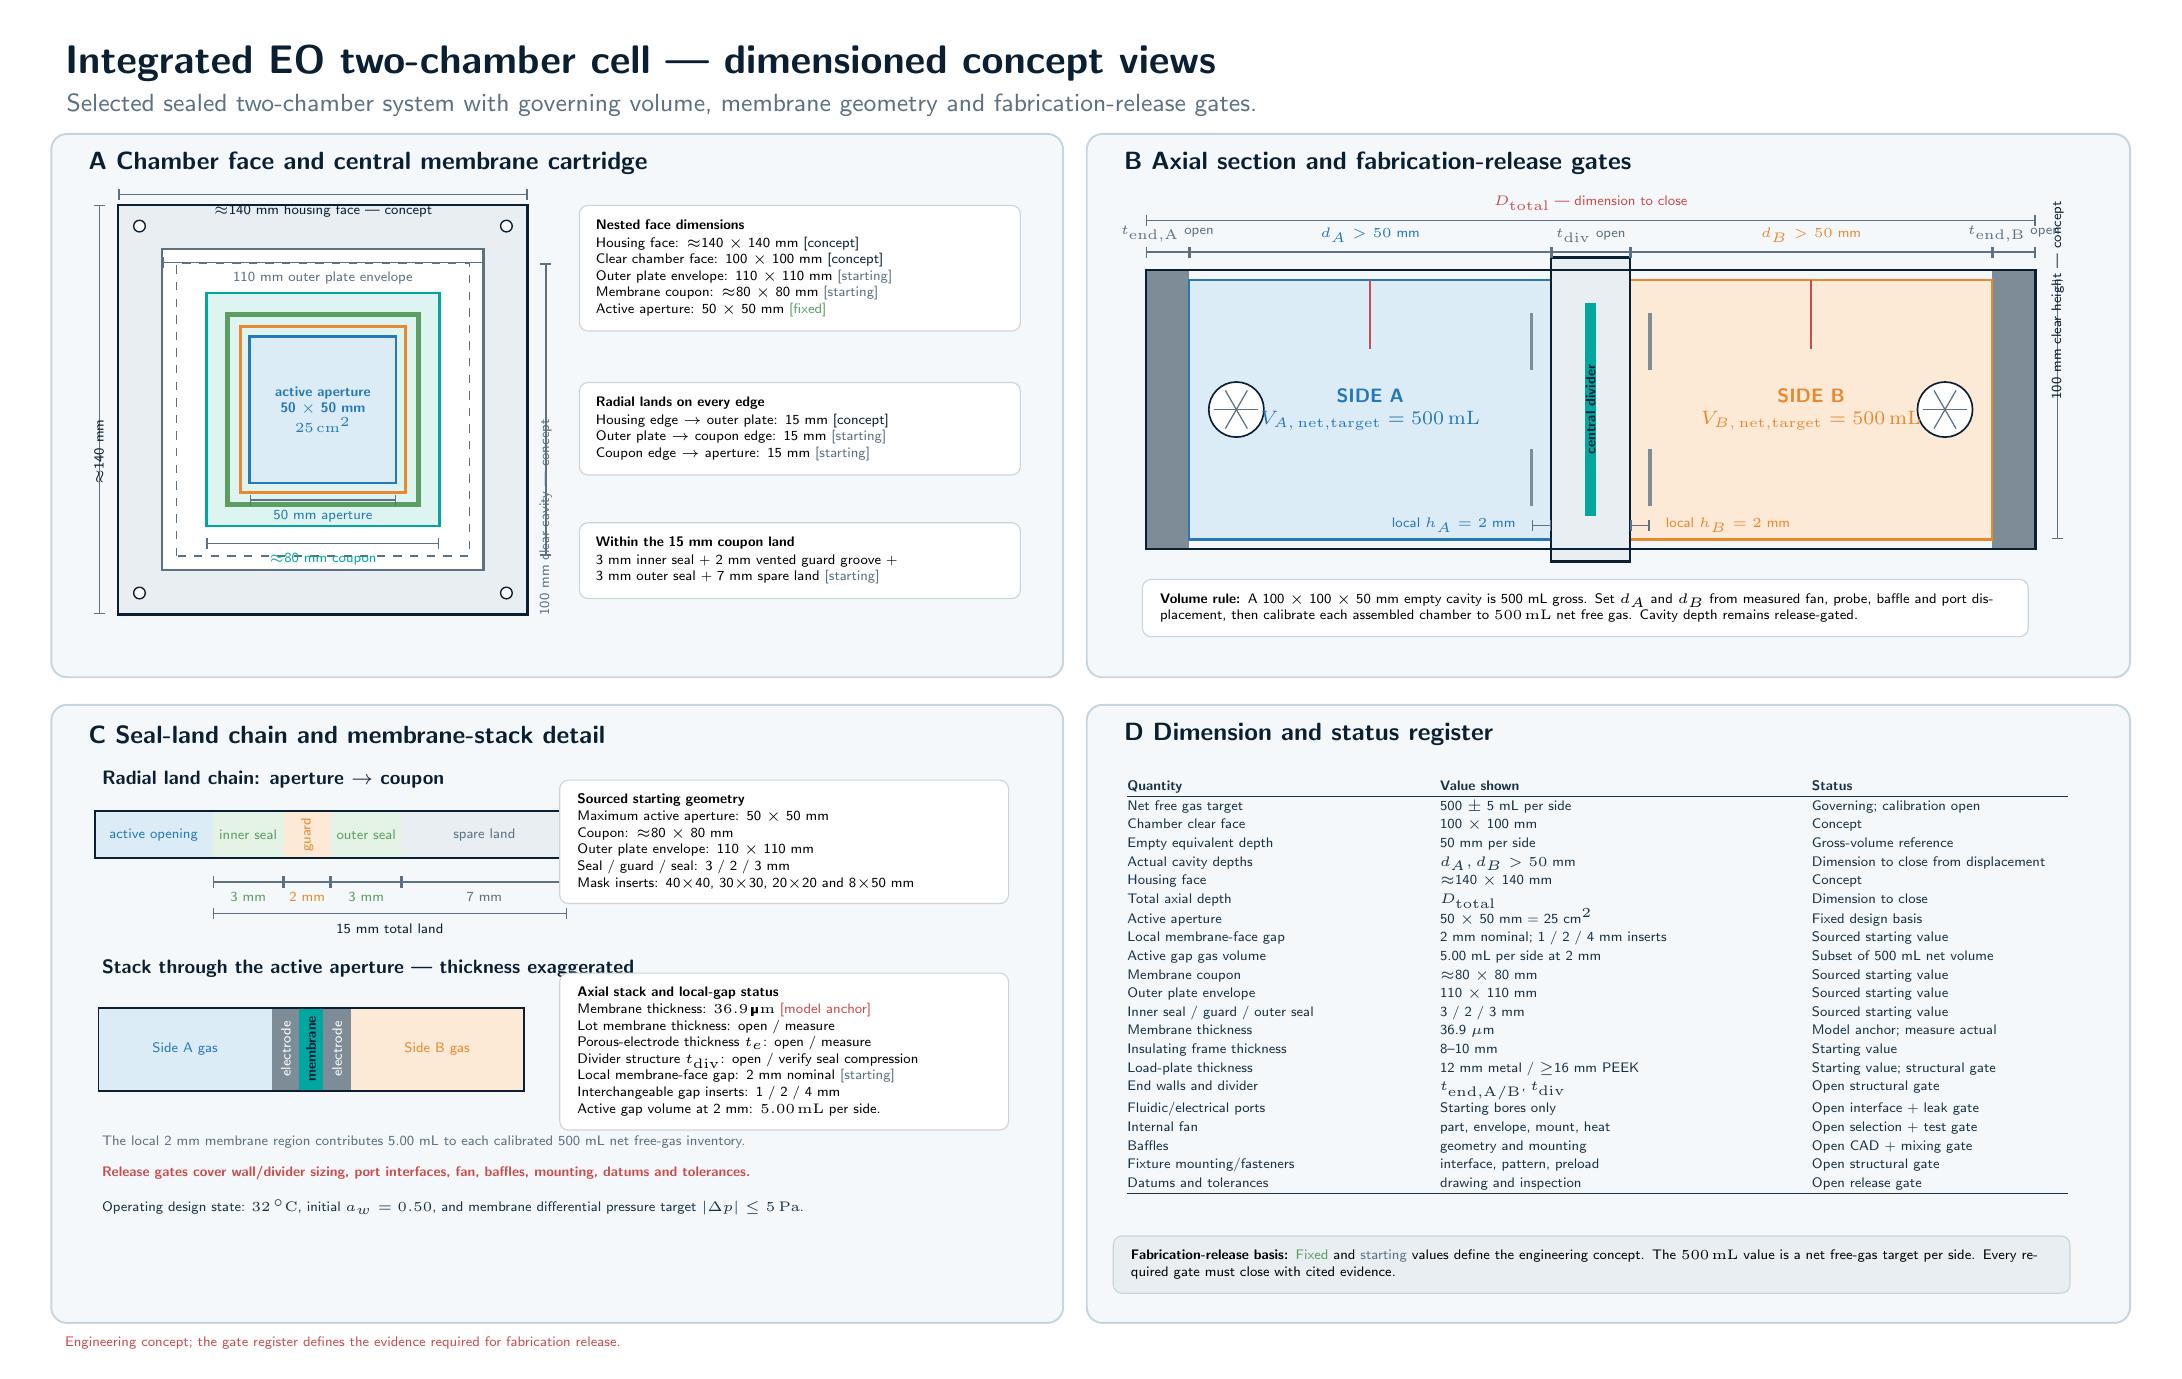
\begin{tikzpicture}[x=1cm,y=1cm]
  \path[use as bounding box] (0,0) rectangle (27,16.8);

  \node[anchor=west, font=\sffamily\bfseries\Large, text=Navy]
    at (0.35,16.35) {Integrated EO two-chamber cell --- dimensioned concept views};
  \node[anchor=west, font=\sffamily\small, text=Slate]
    at (0.37,15.82) {Selected sealed two-chamber system with governing volume, membrane geometry and fabrication-release gates.};

  % ---------------------------------------------------------------------------
  % Panel A: face dimensions
  % ---------------------------------------------------------------------------
  \draw[panel] (0.3,8.55) rectangle (13.15,15.45);
  \node[anchor=west, font=\sffamily\bfseries\small, text=Navy]
    at (0.65,15.08) {A  Chamber face and central membrane cartridge};

  % 140 mm housing, 110 mm frame, 80 mm coupon, 50 mm aperture
  \fill[GreyLight] (1.15,9.35) rectangle (6.35,14.55);
  \draw[Navy, line width=0.9pt] (1.15,9.35) rectangle (6.35,14.55);
  \fill[white] (1.71,9.91) rectangle (5.79,13.99);
  \draw[Slate, line width=0.8pt] (1.71,9.91) rectangle (5.79,13.99);
  % The clear 100 x 100 mm chamber face lies behind the cartridge in this view.
  \draw[Slate, dashed, line width=0.55pt] (1.89,10.09) rectangle (5.61,13.81);
  \fill[TealLight] (2.27,10.47) rectangle (5.23,13.43);
  \draw[Teal, line width=0.8pt] (2.27,10.47) rectangle (5.23,13.43);
  \draw[Green, line width=1.7pt] (2.54,10.74) rectangle (4.96,13.16);
  \draw[Orange, line width=1.1pt] (2.70,10.90) rectangle (4.80,13.00);
  \draw[Green, line width=1.2pt] (2.84,11.04) rectangle (4.66,12.86);
  \fill[BlueLight] (2.82,11.02) rectangle (4.68,12.88);
  \draw[Blue, line width=0.9pt] (2.82,11.02) rectangle (4.68,12.88);
  \node[align=center, font=\sffamily\bfseries\tiny, text=Blue] at (3.75,11.95)
    {active aperture\\50 $\times$ 50 mm\\\SI{25}{cm^2}};

  \foreach \x/\y in {1.42/9.62,6.08/9.62,1.42/14.28,6.08/14.28} {
    \fill[white] (\x,\y) circle (2.1pt);
    \draw[Navy, line width=0.5pt] (\x,\y) circle (2.1pt);
  }

  \draw[dim] (1.15,14.68) -- node[below, font=\sffamily\tiny, text=Navy]
    {$\approx$140 mm housing face --- concept} (6.35,14.68);
  \draw[dim] (0.91,9.35) -- node[left, rotate=90, font=\sffamily\tiny, text=Navy]
    {$\approx$140 mm} (0.91,14.55);
  \draw[dim] (1.71,13.82) -- node[below, font=\sffamily\tiny, text=Slate]
    {110 mm outer plate envelope} (5.79,13.82);
  \draw[dim] (6.58,10.09) -- node[left, rotate=90, font=\sffamily\tiny, text=Slate]
    {100 mm clear cavity --- concept} (6.58,13.81);
  \draw[dim] (2.27,10.25) -- node[below, font=\sffamily\tiny, text=Teal]
    {$\approx$80 mm coupon} (5.23,10.25);
  \draw[dim] (2.82,10.80) -- node[below, font=\sffamily\tiny, text=Blue]
    {50 mm aperture} (4.68,10.80);

  % Dimension chain explanation
  \node[callout, anchor=north west, minimum width=5.60cm, text width=5.18cm]
    at (7.00,14.55) {\textbf{Nested face dimensions}\\[0.2ex]
    Housing face: $\approx$140 $\times$ 140 mm \textcolor{Navy}{[concept]}\\
    Clear chamber face: 100 $\times$ 100 mm \textcolor{Navy}{[concept]}\\
    Outer plate envelope: 110 $\times$ 110 mm \textcolor{Slate}{[starting]}\\
    Membrane coupon: $\approx$80 $\times$ 80 mm \textcolor{Slate}{[starting]}\\
    Active aperture: 50 $\times$ 50 mm \textcolor{Green}{[fixed]}};

  \node[callout, anchor=north west, minimum width=5.60cm, text width=5.18cm]
    at (7.00,12.30) {\textbf{Radial lands on every edge}\\[0.2ex]
    Housing edge $\rightarrow$ outer plate: 15 mm \textcolor{Navy}{[concept]}\\
    Outer plate $\rightarrow$ coupon edge: 15 mm \textcolor{Slate}{[starting]}\\
    Coupon edge $\rightarrow$ aperture: 15 mm \textcolor{Slate}{[starting]}};

  \node[callout, anchor=north west, minimum width=5.60cm, text width=5.18cm]
    at (7.00,10.52) {\textbf{Within the 15 mm coupon land}\\[0.2ex]
    3 mm inner seal + 2 mm vented guard groove +\\
    3 mm outer seal + 7 mm spare land \textcolor{Slate}{[starting]}};

  % ---------------------------------------------------------------------------
  % Panel B: axial dimensions
  % ---------------------------------------------------------------------------
  \draw[panel] (13.45,8.55) rectangle (26.7,15.45);
  \node[anchor=west, font=\sffamily\bfseries\small, text=Navy]
    at (13.80,15.08) {B  Axial section and fabrication-release gates};

  \fill[Grey] (14.20,10.18) rectangle (14.75,13.72);
  \fill[BlueLight] (14.75,10.30) rectangle (19.35,13.60);
  \fill[GreyLight] (19.35,10.02) rectangle (20.35,13.88);
  \fill[Teal] (19.78,10.60) rectangle (19.92,13.30);
  \fill[OrangeLight] (20.35,10.30) rectangle (24.95,13.60);
  \fill[Grey] (24.95,10.18) rectangle (25.50,13.72);
  \draw[Navy, line width=0.8pt] (14.20,10.18) rectangle (25.50,13.72);
  \draw[Blue, line width=0.8pt] (14.75,10.30) rectangle (19.35,13.60);
  \draw[Orange, line width=0.8pt] (20.35,10.30) rectangle (24.95,13.60);
  \draw[Navy, line width=0.8pt] (19.35,10.02) rectangle (20.35,13.88);

  % Fans, probes and baffles
  \draw[Navy, line width=0.6pt, fill=white] (15.35,11.95) circle (0.35);
  \draw[Navy, line width=0.6pt, fill=white] (24.35,11.95) circle (0.35);
  \foreach \a in {0,60,...,300} {
    \draw[Slate, line width=0.45pt] (15.35,11.95) -- ++(\a:0.28);
    \draw[Slate, line width=0.45pt] (24.35,11.95) -- ++(\a:0.28);
  }
  \draw[Red, line width=0.55pt] (17.05,13.60) -- (17.05,12.72);
  \draw[Red, line width=0.55pt] (22.65,13.60) -- (22.65,12.72);
  % Flow guides create the local membrane-face region; spacing is schematic here.
  \draw[Grey, line width=1.3pt] (19.10,10.72) -- (19.10,11.45);
  \draw[Grey, line width=1.3pt] (19.10,12.45) -- (19.10,13.18);
  \draw[Grey, line width=1.3pt] (20.60,10.72) -- (20.60,11.45);
  \draw[Grey, line width=1.3pt] (20.60,12.45) -- (20.60,13.18);
  \draw[dim] (19.10,10.48) -- (19.35,10.48);
  \node[anchor=east, font=\sffamily\tiny, text=Blue] at (19.02,10.48)
    {local $h_A=2$ mm};
  \draw[dim] (20.35,10.48) -- (20.60,10.48);
  \node[anchor=west, font=\sffamily\tiny, text=Orange] at (20.68,10.48)
    {local $h_B=2$ mm};

  \node[align=center, font=\sffamily\bfseries\scriptsize, text=Blue] at (17.05,11.95)
    {SIDE A\\$V_{A,\,\rm net,target}=\SI{500}{mL}$};
  \node[align=center, font=\sffamily\bfseries\scriptsize, text=Orange] at (22.65,11.95)
    {SIDE B\\$V_{B,\,\rm net,target}=\SI{500}{mL}$};
  \node[rotate=90, font=\sffamily\bfseries\tiny, text=Navy] at (19.85,11.95)
    {central divider};

  \draw[dim] (14.20,14.35) -- node[above, font=\sffamily\tiny, text=Red]
    {$D_{\rm total}$ --- dimension to close} (25.50,14.35);
  \draw[dim] (14.20,13.95) -- node[above, font=\sffamily\tiny, text=Slate]
    {$t_{\rm end,A}$ open} (14.75,13.95);
  \draw[dim] (14.75,13.95) -- node[above, font=\sffamily\tiny, text=Blue]
    {$d_A>50$ mm} (19.35,13.95);
  \draw[dim] (19.35,13.95) -- node[above, font=\sffamily\tiny, text=Slate]
    {$t_{\rm div}$ open} (20.35,13.95);
  \draw[dim] (20.35,13.95) -- node[above, font=\sffamily\tiny, text=Orange]
    {$d_B>50$ mm} (24.95,13.95);
  \draw[dim] (24.95,13.95) -- node[above, font=\sffamily\tiny, text=Slate]
    {$t_{\rm end,B}$ open} (25.50,13.95);
  \draw[dim] (25.78,10.30) -- node[right, rotate=90, font=\sffamily\tiny, text=Navy]
    {100 mm clear height --- concept} (25.78,13.60);

  \node[callout, anchor=north west, minimum width=11.25cm, text width=10.80cm]
    at (14.15,9.80) {\textbf{Volume rule:} A 100 $\times$ 100 $\times$ 50 mm empty cavity is 500 mL gross. Set $d_A$ and $d_B$ from measured fan, probe, baffle and port displacement, then calibrate each assembled chamber to \SI{500}{mL} net free gas. Cavity depth remains release-gated.};

  % ---------------------------------------------------------------------------
  % Panel C: seal and membrane detail
  % ---------------------------------------------------------------------------
  \draw[panel] (0.3,0.35) rectangle (13.15,8.20);
  \node[anchor=west, font=\sffamily\bfseries\small, text=Navy]
    at (0.65,7.82) {C  Seal-land chain and membrane-stack detail};

  \node[anchor=west, font=\sffamily\bfseries\scriptsize, text=Navy] at (0.82,7.25)
    {Radial land chain: aperture $\rightarrow$ coupon};
  \fill[BlueLight] (0.85,6.25) rectangle (2.35,6.85);
  \fill[GreenLight] (2.35,6.25) rectangle (3.25,6.85);
  \fill[OrangeLight] (3.25,6.25) rectangle (3.85,6.85);
  \fill[GreenLight] (3.85,6.25) rectangle (4.75,6.85);
  \fill[GreyLight] (4.75,6.25) rectangle (6.85,6.85);
  \draw[Navy, line width=0.65pt] (0.85,6.25) rectangle (6.85,6.85);
  \node[font=\sffamily\tiny, text=Blue] at (1.60,6.55) {active opening};
  \node[font=\sffamily\tiny, text=Green] at (2.80,6.55) {inner seal};
  \node[font=\sffamily\tiny, text=Orange, rotate=90] at (3.55,6.55) {guard};
  \node[font=\sffamily\tiny, text=Green] at (4.30,6.55) {outer seal};
  \node[font=\sffamily\tiny, text=Slate] at (5.80,6.55) {spare land};
  \draw[dim] (2.35,5.95) -- node[below, font=\sffamily\tiny, text=Green] {3 mm} (3.25,5.95);
  \draw[dim] (3.25,5.95) -- node[below, font=\sffamily\tiny, text=Orange] {2 mm} (3.85,5.95);
  \draw[dim] (3.85,5.95) -- node[below, font=\sffamily\tiny, text=Green] {3 mm} (4.75,5.95);
  \draw[dim] (4.75,5.95) -- node[below, font=\sffamily\tiny, text=Slate] {7 mm} (6.85,5.95);
  \draw[dim] (2.35,5.55) -- node[below, font=\sffamily\tiny, text=Navy]
    {15 mm total land} (6.85,5.55);

  \node[anchor=west, font=\sffamily\bfseries\scriptsize, text=Navy] at (0.82,4.85)
    {Stack through the active aperture --- thickness exaggerated};
  \fill[BlueLight] (0.90,3.30) rectangle (3.10,4.35);
  \fill[Grey] (3.10,3.30) rectangle (3.45,4.35);
  \fill[Teal] (3.45,3.30) rectangle (3.75,4.35);
  \fill[Grey] (3.75,3.30) rectangle (4.10,4.35);
  \fill[OrangeLight] (4.10,3.30) rectangle (6.30,4.35);
  \draw[Navy, line width=0.65pt] (0.90,3.30) rectangle (6.30,4.35);
  \node[font=\sffamily\tiny, text=Blue] at (2.00,3.83) {Side A gas};
  \node[font=\sffamily\tiny, text=Orange] at (5.20,3.83) {Side B gas};
  \node[rotate=90, font=\sffamily\tiny, text=white] at (3.28,3.83) {electrode};
  \node[rotate=90, font=\sffamily\bfseries\tiny, text=Navy] at (3.60,3.83) {membrane};
  \node[rotate=90, font=\sffamily\tiny, text=white] at (3.93,3.83) {electrode};

  \node[callout, anchor=north west, minimum width=5.70cm, text width=5.25cm]
    at (6.75,7.25) {\textbf{Sourced starting geometry}\\
    Maximum active aperture: 50 $\times$ 50 mm\\
    Coupon: $\approx$80 $\times$ 80 mm\\
    Outer plate envelope: 110 $\times$ 110 mm\\
    Seal / guard / seal: 3 / 2 / 3 mm\\
    Mask inserts: 40$\times$40, 30$\times$30, 20$\times$20 and 8$\times$50 mm};

  \node[callout, anchor=north west, minimum width=5.70cm, text width=5.25cm]
    at (6.75,4.80) {\textbf{Axial stack and local-gap status}\\
    Membrane thickness: \SI{36.9}{\micro\metre} \textcolor{Red}{[model anchor]}\\
    Lot membrane thickness: open / measure\\
    Porous-electrode thickness $t_e$: open / measure\\
    Divider structure $t_{\rm div}$: open / verify seal compression\\
    Local membrane-face gap: 2 mm nominal \textcolor{Slate}{[starting]}\\
    Interchangeable gap inserts: 1 / 2 / 4 mm\\
    Active gap volume at 2 mm: \SI{5.00}{mL} per side.};

  \node[anchor=west, font=\sffamily\tiny, text=Slate] at (0.82,2.65)
    {The local 2 mm membrane region contributes 5.00 mL to each calibrated 500 mL net free-gas inventory.};
  \node[anchor=west, font=\sffamily\bfseries\tiny, text=Red] at (0.82,2.25)
    {Release gates cover wall/divider sizing, port interfaces, fan, baffles, mounting, datums and tolerances.};
  \node[anchor=west, font=\sffamily\tiny, text=Ink] at (0.82,1.82)
    {Operating design state: \SI{32}{\celsius}, initial $a_w=0.50$, and membrane differential pressure target $|\Delta p|\leq\SI{5}{Pa}$.};

  % ---------------------------------------------------------------------------
  % Panel D: status register
  % ---------------------------------------------------------------------------
  \draw[panel] (13.45,0.35) rectangle (26.7,8.20);
  \node[anchor=west, font=\sffamily\bfseries\small, text=Navy]
    at (13.80,7.82) {D  Dimension and status register};

  \node[anchor=north west, font=\sffamily\tiny, text=Ink] at (13.78,7.40) {\renewcommand{\arraystretch}{1.12}
  \begin{tabular}{@{}>{\raggedright\arraybackslash}p{3.55cm}>{\raggedright\arraybackslash}p{4.30cm}>{\raggedright\arraybackslash}p{3.25cm}@{}}
  \textbf{Quantity} & \textbf{Value shown} & \textbf{Status} \\\hline
  Net free gas target & 500 $\pm$ 5 mL per side & Governing; calibration open \\
  Chamber clear face & 100 $\times$ 100 mm & Concept \\
  Empty equivalent depth & 50 mm per side & Gross-volume reference \\
  Actual cavity depths & $d_A,d_B>50$ mm & Dimension to close from displacement \\
  Housing face & $\approx$140 $\times$ 140 mm & Concept \\
  Total axial depth & $D_{\rm total}$ & Dimension to close \\
  Active aperture & 50 $\times$ 50 mm = 25 cm$^2$ & Fixed design basis \\
  Local membrane-face gap & 2 mm nominal; 1 / 2 / 4 mm inserts & Sourced starting value \\
  Active gap gas volume & 5.00 mL per side at 2 mm & Subset of 500 mL net volume \\
  Membrane coupon & $\approx$80 $\times$ 80 mm & Sourced starting value \\
  Outer plate envelope & 110 $\times$ 110 mm & Sourced starting value \\
  Inner seal / guard / outer seal & 3 / 2 / 3 mm & Sourced starting value \\
  Membrane thickness & 36.9 $\mu$m & Model anchor; measure actual \\
  Insulating frame thickness & 8--10 mm & Starting value \\
  Load-plate thickness & 12 mm metal / $\geq$16 mm PEEK & Starting value; structural gate \\
  End walls and divider & $t_{\rm end,A/B}$, $t_{\rm div}$ & Open structural gate \\
  Fluidic/electrical ports & Starting bores only & Open interface + leak gate \\
  Internal fan & part, envelope, mount, heat & Open selection + test gate \\
  Baffles & geometry and mounting & Open CAD + mixing gate \\
  Fixture mounting/fasteners & interface, pattern, preload & Open structural gate \\
  Datums and tolerances & drawing and inspection & Open release gate \\\hline
  \end{tabular}};

  \node[callout, anchor=south west, minimum width=12.15cm, text width=11.70cm,
    fill=GreyLight] at (13.78,0.72) {\textbf{Fabrication-release basis:} \textcolor{Green}{Fixed} and \textcolor{Slate}{starting} values define the engineering concept. The \SI{500}{mL} value is a net free-gas target per side. Every required gate must close with cited evidence.};

  \node[anchor=west, font=\sffamily\tiny, text=Red] at (0.35,0.10)
    {Engineering concept; the gate register defines the evidence required for fabrication release.};

\end{tikzpicture}
\end{document}
